% Learned page replacement for xv6: the traces2 study.
%
% Build (from report/slides):  pdflatex ml_results.tex && pdflatex ml_results.tex
%
% Every number here comes from report/results2/ (tables/*.tex are generated
% by tools/ml2/tables.py, figures by tools/ml2/figures.py); the prose is in
% report/ML_REPORT.md.

\documentclass[10pt,aspectratio=169]{beamer}

\usetheme{metropolis}
\usepackage[T1]{fontenc}
\usepackage{lmodern}
\usepackage{booktabs}
\usepackage{multirow}
\usepackage{xcolor}
\usepackage{graphicx}
\usepackage{tikz}
\usetikzlibrary{arrows.meta,positioning}

\metroset{sectionpage=progressbar, numbering=fraction, progressbar=frametitle}

\definecolor{accent}{HTML}{2C6E8F}
\definecolor{warn}{HTML}{B5540A}
\definecolor{good}{HTML}{2E7D4F}
\setbeamercolor{alerted text}{fg=warn}
\setbeamercolor{frametitle}{bg=accent}
\setbeamercolor{progress bar}{fg=accent}

\newcommand{\good}[1]{\textcolor{good}{#1}}
\newcommand{\warn}[1]{\textcolor{warn}{#1}}
\newcommand{\tbl}[1]{{\scriptsize\input{tables/#1.tex}}}
\graphicspath{{../figures2/}}

\title{Learned Page Replacement for xv6}
\subtitle{Training on verified reference streams, and what a kernel can actually use}
\date{\texttt{traces2} study --- report/ML\_REPORT.md}

\begin{document}

\maketitle

% ------------------------------------------------------------------ question
\section{The question}

\begin{frame}{Can a learned model replace the kernel's page-replacement policy?}
  \small
  Train on memory workloads, integrate the model into xv6, measure it --- a
  precursor to Linux.

  \medskip
  \textbf{Three constraints shape everything:}
  \begin{enumerate}
    \item \textbf{No floating point in xv6.} Anything learned must run in integers.
    \item \textbf{A kernel never sees memory accesses.} The MMU handles loads and
      stores; the kernel sees faults and the accessed/dirty bits it can read at a
      scan. Same in Linux for anonymous memory.
    \item \textbf{Decisions compound.} Policies can only be compared by replaying
      whole reference streams --- all results are fault counts, not prediction accuracy.
  \end{enumerate}

  \medskip
  So every model is trained on three \textbf{feature tiers}: what only an oracle
  trace has, what a kernel observes, and what a kernel can cheaply book-keep ---
  the first is an \emph{ablation}, not a deployable result.
\end{frame}

\begin{frame}{Pipeline}
  \centering
  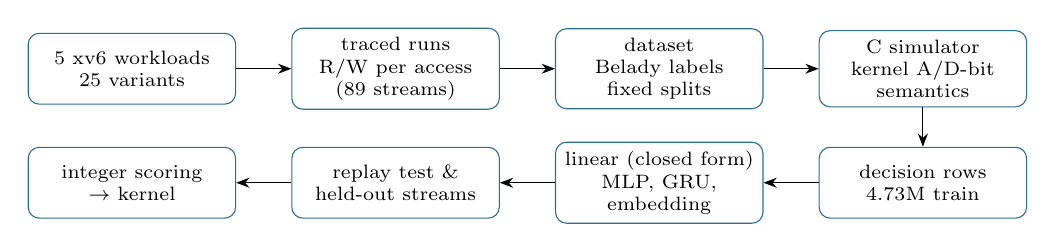
\begin{tikzpicture}[node distance=5mm and 7mm, every node/.style={font=\scriptsize,
      draw=accent, rounded corners, align=center, minimum height=9mm, text width=24mm},
      >={Stealth}]
    \node (wl) {5 xv6 workloads\\25 variants};
    \node[right=of wl] (tr) {traced runs\\R/W per access\\(89 streams)};
    \node[right=of tr] (ds) {dataset\\Belady labels\\fixed splits};
    \node[right=of ds] (sim) {C simulator\\kernel A/D-bit\\semantics};
    \node[below=of sim] (rec) {decision rows\\4.73M train};
    \node[left=of rec] (tr2) {linear (closed form)\\MLP, GRU, embedding};
    \node[left=of tr2] (ev) {replay test \&\\held-out streams};
    \node[left=of ev] (int) {integer scoring\\$\to$ kernel};
    \draw[->] (wl) -- (tr); \draw[->] (tr) -- (ds); \draw[->] (ds) -- (sim);
    \draw[->] (sim) -- (rec); \draw[->] (rec) -- (tr2); \draw[->] (tr2) -- (ev);
    \draw[->] (ev) -- (int);
  \end{tikzpicture}
\end{frame}

% ------------------------------------------------------------------ traces
\section{How the traces were made}

\begin{frame}{The workloads}
  \scriptsize
  \begin{tabular}{p{2.1cm}p{5.2cm}p{5.4cm}}
    \toprule
    Workload & Models & Why no single heuristic wins \\
    \midrule
    \texttt{btreebench} & B+tree (SQLite pager): insert, lookup, scan, mixed, WAL & lookups favour frequency, inserts recency, scans sequential \\
    \texttt{kvbench} & Zipfian hash table (Redis): YCSB modes A/B/C/D/F, rehash, value sizes & hot set rotates: old-hot pages must go cold \\
    \texttt{graphbench} & BFS + fixed-point PageRank on a scale-free graph & data-dependent frontier; hubs revisited each iteration \\
    \texttt{sortbench} & bottom-up merge sort & deliberately sequential (calibration) \\
    \texttt{matmulbench} & naive vs.\ blocked matrix multiply & locality contrast, tiny working sets \\
    \bottomrule
  \end{tabular}
\end{frame}

\begin{frame}{Collecting a complete, verified reference string}
  \small
  \begin{itemize}
    \item Every arena access goes through \texttt{vmbench\_trace\_ref(vpn, access)}:
      one line \texttt{R <vpn>} or \texttt{W <vpn>} per access --- \emph{every}
      touch, not just faults. No default access type: an unmarked site does not compile.
    \item A reference string does not depend on memory size, so each stream is
      \textbf{one run at a generous margin}; capacities are chosen in simulation.
    \item 25 variants $\times$ seeds = \textbf{89 streams} + 22 repeats, 6 parallel lanes.
      A stream counts only if the run passed and the file matches
      \texttt{TRACEEND refs=N bytes=M} exactly.
    \item All 111 runs passed; all 22 repeats \good{byte-identical}.
    \item Checked against the kernel: FIFO replay reproduces its evictions with
      3--5 untraced frames ($-0.1\%$); W marks predict its \texttt{page\_writes}.
  \end{itemize}
\end{frame}

\begin{frame}{Why the older traces were dropped}
  \small
  Two of the six old captures were wrong (found by AU5TRA, commit \texttt{9d36525}):
  \begin{itemize}
    \item \textbf{graphbench} traced only the edge array --- BFS \texttt{visited[]}
      and PageRank \texttt{rank[]} were never recorded: \warn{57\% of references,
      667 of 2000 pages missing}.
    \item \textbf{lzwbench}'s trace hit xv6's maximum file size and
      \warn{silently lost $\sim$42\% of the run} while still printing PASS.
  \end{itemize}
  \medskip
  The earlier report's two headline wins (graph $-4.3\%$, lzw $-24\%$ vs.\ Clock)
  were on these two traces. \textbf{They should not be cited.} Everything here
  uses the new streams.
\end{frame}

\begin{frame}{The dataset and its splits}
  \small
  \begin{columns}[T]
    \column{.5\textwidth}
    Per reference: \texttt{vpn}, \texttt{write}, \texttt{next\_use}.\\
    \texttt{next\_use} = distance to the page's next access --- what Belady evicts by.
    A \textbf{label only}, never an input.

    \medskip
    \textbf{held-out}: variants never trained on\\
    \quad kv-F, btree-scan, graph-bfs2000, sort-n60000, matmul-128\\
    \textbf{test}: last seed of every other variant\\
    \textbf{val}: second-to-last seed
    \column{.45\textwidth}
    \centering
    \begin{tabular}{lrr}
      \toprule
      Split & Streams & References \\
      \midrule
      train & 41 & 45.5M \\
      val & 15 & 23.6M \\
      test & 15 & 23.6M \\
      held-out & 18 & 30.6M \\
      \bottomrule
    \end{tabular}
  \end{columns}
\end{frame}

% ------------------------------------------------------------------ method
\section{Features, models, method}

\begin{frame}{Three feature tiers}
  \scriptsize
  \begin{tabular}{llp{5.3cm}p{3.4cm}}
    \toprule
    Tier & Feature & Definition & Linux analogue \\
    \midrule
    \warn{F (oracle)} & \texttt{rec} & references since last access & --- \\
     & \texttt{freq} & exact access count & --- \\
     & \texttt{sd} & distinct pages since last access & --- \\
     & \texttt{wr} & fraction of accesses that wrote & --- \\
    \midrule
    \textcolor{accent}{K (kernel)} & \texttt{ref} & accessed bit at this scan & referenced / young bit \\
     & \texttt{aging} & 8-bit aging counter (xv6 Aging) & --- \\
     & \texttt{sfreq} & scans that found it accessed & DAMON \texttt{nr\_accesses}, MGLRU tiers \\
     & \texttt{idle} & scans since last found accessed & MGLRU generations, DAMON age \\
     & \texttt{age} & scans since loaded & --- \\
     & \texttt{dirty} & dirty bit & \texttt{PG\_dirty} \\
    \midrule
    \good{K+ (bookkeeping)} & \texttt{refaults} & times evicted and faulted back & \multirow{2}{*}{\texttt{mm/workingset.c} shadow entries} \\
     & \texttt{rdist} & evictions between eviction and refault & \\
    \bottomrule
  \end{tabular}
\end{frame}

\begin{frame}{Simulator, validated before use}
  \small
  \texttt{tools/ml2/pagesim.c}: replays a stream from empty memory; FIFO, Clock, Aging,
  LRU, exact/decayed LFU, Belady, and any learned scorer. Accessed/dirty bits follow
  the kernel (a fault sets \texttt{PTE\_A}, and \texttt{PTE\_D} on a write).
  \begin{itemize}
    \item FIFO, LRU, Belady equal AU5TRA's independent \texttt{baselines.tsv} on
      \good{all 534 stream $\times$ capacity cells}.
    \item Clock/Aging/decayed LFU match a naive Python re-implementation in faults
      and writebacks; all kernel features match on 11,792 evictions $\times$ 53 candidates.
    \item The C scorer reproduces every trained model (max error $\le 3\times10^{-5}$).
  \end{itemize}
  \medskip
  Two corrections to the earlier study: its ``stack distance'' counted first-ever
  touches, not distinct pages (true stack distance orders pages exactly like LRU);
  and pooled correlation misled --- what matters is ranking \emph{within} a decision.
\end{frame}

\begin{frame}{Training on decisions}
  \small
  \begin{itemize}
    \item Replay every train/val stream at 5, 10, 20\% of its distinct pages under
      LRU; at sampled evictions record 32 resident candidates --- Belady's choice,
      the 4 most recently used, and random others --- with all 12 features and
      $\log(1 + \text{distance to next use})$.
    \item \textbf{4.73M rows over 357K eviction decisions}; 0.84M validation rows.
    \item Models: \textbf{linear} (closed form, any subset), \textbf{MLP} 2$\times$32,
      a \textbf{ranking loss} (softmax over one decision's candidates),
      \textbf{GRU} over the last 8 access intervals, \textbf{cross-page embedding}.
    \item Scopes: one model per workload, and one \textbf{global} model --- the
      realistic one: a kernel does not know which program is running.
    \item \textbf{Every combination}: 300 feature sets $\times$ 6 scopes =
      28,800 full replays at 10\%.
    \item \textbf{Nested selection on validation}: top-5 subsets per tier $\times$
      probation $\{0,1,2,4\}$ at 5/10/20\%; only the winner is run on test and held-out.
  \end{itemize}
\end{frame}

% ------------------------------------------------------------------ results
\section{Results}

\begin{frame}{What xv6 can already do: the classical policies}
  \centering
  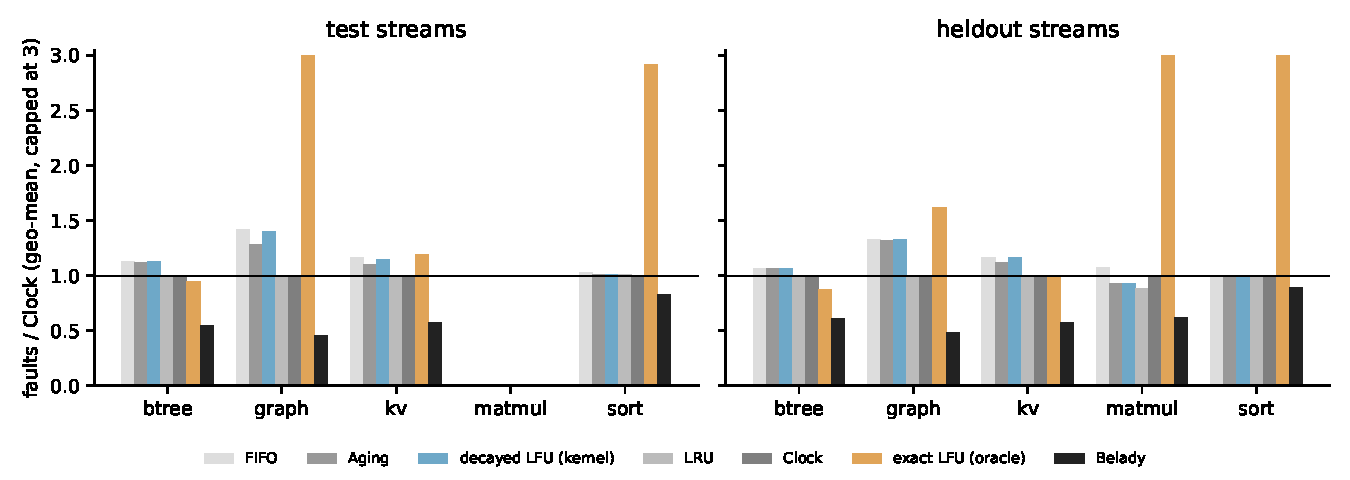
\includegraphics[width=.92\textwidth]{classical.pdf}

  \footnotesize Faults relative to Clock (xv6's best), geo-mean over streams $\times$ 5/10/20\%.
  Aging $\approx$ FIFO; exact LFU wins on btree and is catastrophic elsewhere;
  Belady needs 43--54\% fewer faults on btree/kv/graph.
\end{frame}

\begin{frame}{Which features carry signal --- within one eviction}
  \begin{columns}[c]
    \column{.5\textwidth}
    \centering
    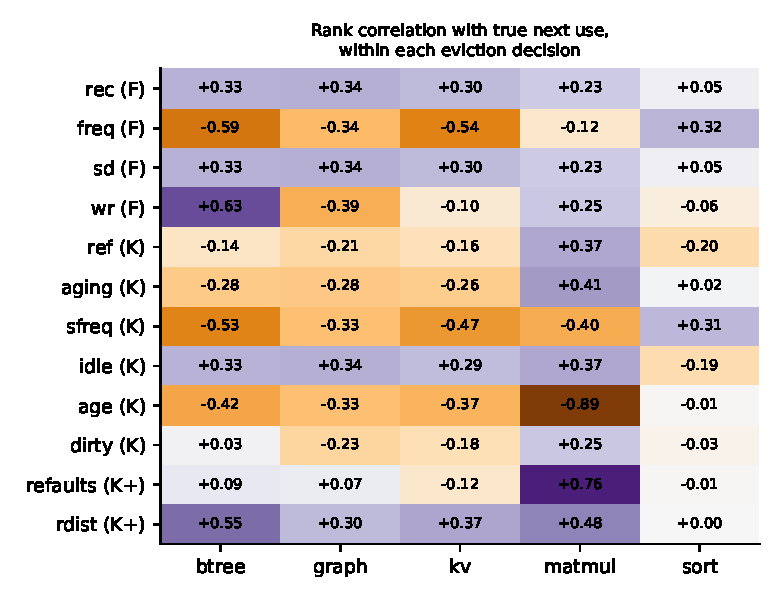
\includegraphics[width=\textwidth]{diagnostics.pdf}
    \column{.48\textwidth}
    \small
    Rank correlation with the true next use, \emph{among the candidates of one decision}.
    \begin{itemize}
      \item Sampled access count \texttt{sfreq} ($-0.45$) $\approx$ exact count \texttt{freq} ($-0.52$).
      \item Refault distance \texttt{rdist} --- Linux already measures it --- is as strong.
      \item Recency and true stack distance are identical within a decision.
      \item Pooled correlation misleads: \texttt{rec} on sort is $+0.87$ pooled, $+0.05$ within decisions.
    \end{itemize}
  \end{columns}
\end{frame}

\begin{frame}{Every full-stream combination (15 subsets)}
  \centering
  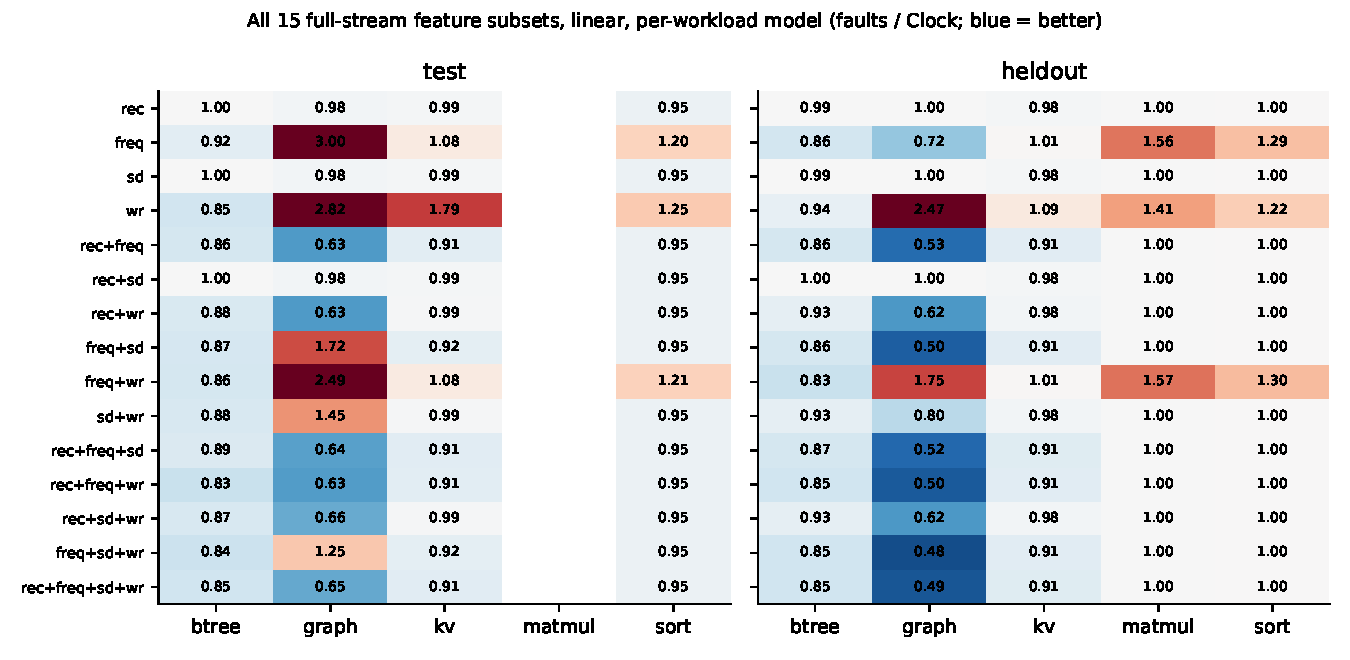
\includegraphics[width=.86\textwidth]{f_subsets_workload.pdf}

  \footnotesize One feature is never enough; \textbf{recency + frequency} is the pair that matters.
\end{frame}

\begin{frame}{All 255 kernel-observable combinations}
  \centering
  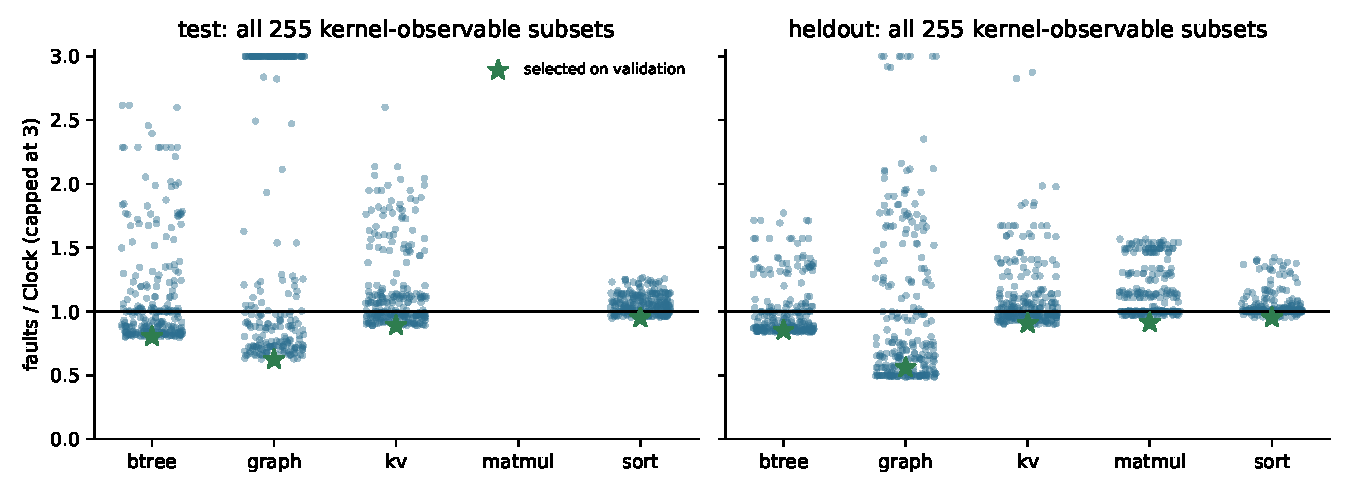
\includegraphics[width=.8\textwidth]{kk_subsets.pdf}

  \tbl{kksubsets_workload_test}
\end{frame}

\begin{frame}{What each kernel feature is worth}
  \begin{columns}[c]
    \column{.55\textwidth}
    \centering
    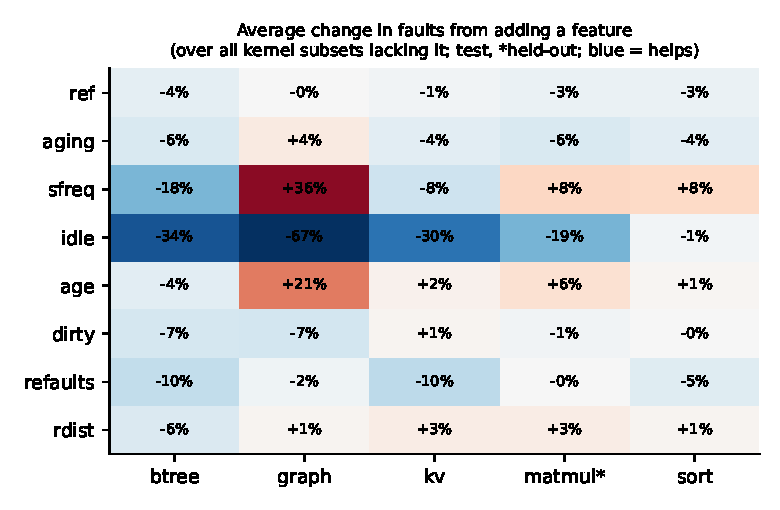
\includegraphics[width=\textwidth]{marginal.pdf}
    \column{.43\textwidth}
    \small
    Median change in faults when a feature is added to a subset that lacks it.
    \begin{itemize}
      \item \texttt{idle} --- scans since last found accessed --- dominates:
        \good{$-71\%$ graph, $-29\%$ btree, $-20\%$ kv}.
      \item That is exactly what Linux's MGLRU generations and DAMON age track.
      \item Refault count helps btree/kv/sort.
    \end{itemize}
  \end{columns}
\end{frame}

\begin{frame}{What went wrong first: evicting the page being streamed}
  \small
  v1 recorded Belady's choice + 31 \emph{uniform} candidates per decision.
  On PageRank almost every model was \warn{$\geq 3\times$ Clock} --- even one
  trained on PageRank alone; three DAgger rounds did not help.
  \begin{itemize}
    \item At its own decisions: \warn{97\% of victims loaded at the previous fault},
      next use a median \textbf{16 references} away (Belady's choice: $\sim$300 refs stale).
    \item Uniform samples of a 167-page resident set almost never contain the
      page just touched --- no model ever saw ``just used, keep it''.
    \item Same pathology as the kernel LFU livelock, by a different route.
  \end{itemize}
  \medskip
  \textbf{Fixes, both chosen on validation:} record the 4 most recently used
  candidates too; \textbf{probation} --- a page loaded $<p$ scans ago is not
  evicted while an older one exists (Clock's second chance). Graph: $0.81 \to 0.61$;
  matmul prefers $p=0$ (5 frames), so $p$ is chosen per scope.
\end{frame}

\begin{frame}{Headline: validation-selected models, per workload}
  \centering
  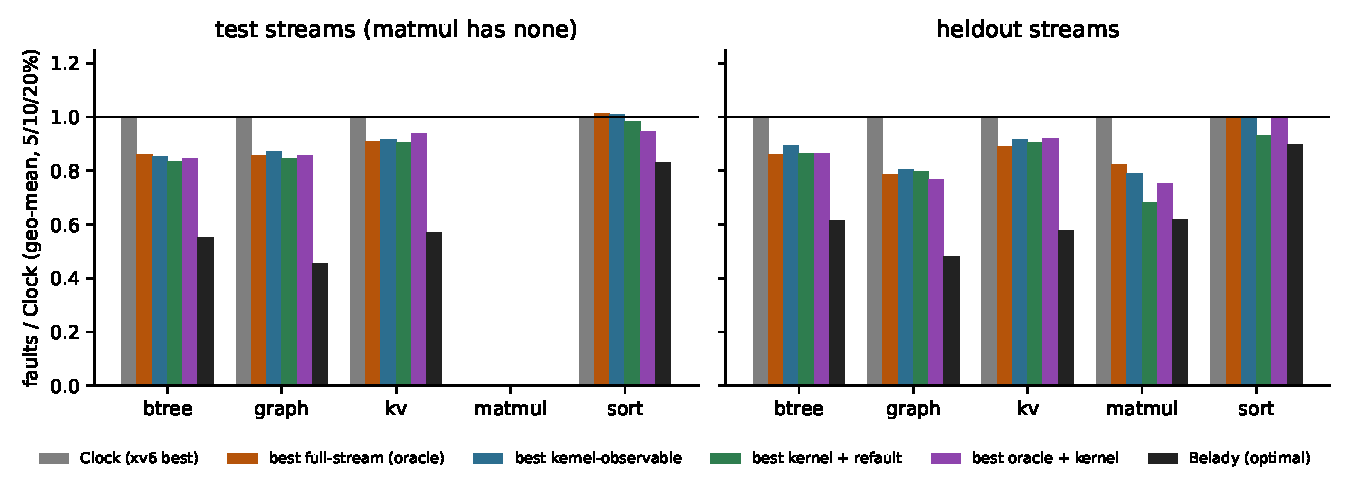
\includegraphics[width=.92\textwidth]{tiers_workload.pdf}

  \footnotesize Subset and probation chosen on validation only; geo-mean over 5/10/20\%.
\end{frame}

\begin{frame}{Headline numbers}
  \centering\tbl{headline_workload_test}

  \medskip\tbl{headline_workload_heldout}

  \medskip\scriptsize faults / Clock (share of the Clock$\to$Belady gap closed)
\end{frame}

\begin{frame}{The kernel's own signals are enough}
  \small
  \begin{itemize}
    \item With only accessed/dirty-bit scan history + refault bookkeeping, the
      selected policy \good{beats Clock on every workload}, on unseen seeds
      \emph{and} unseen variants:\\
      btree $-17/-14\%$, graph $-15/-20\%$, kv $-10/-10\%$, matmul $-32\%$, sort $-2/-7\%$
      (test / held-out).
    \item The oracle features are within $\pm1.5\%$ of it on btree/graph/kv and
      behind on matmul and sort: \textbf{what a kernel cannot see is not what
      limits a learned policy here.}
    \item Refault bookkeeping helps in all 9 workload $\times$ split cells.
    \item Held-out variants generalise as well as unseen seeds.
    \item \textbf{One global model} (the deployable case) still beats Clock in 8 of 9 cells,
      keeping most of the gain on btree/graph/kv.
  \end{itemize}
\end{frame}

\begin{frame}{Fewer disk writes, not just fewer faults}
  \centering\tbl{writebacks}

  \medskip\small
  The selected models use the dirty bit: graph needs \good{58--66\% fewer page
  writes} than Clock (Belady, which ignores writes: 70--74\%).
\end{frame}

\begin{frame}{Where it does not help: capacity dependence}
  \centering\tbl{bycap_KpKp}

  \medskip\small
  Graph's gain is concentrated at 10\%; at 5\% and 20\% no linear model gets below
  0.93 even though Belady has large headroom --- including models trained only on
  that capacity.
\end{frame}

\begin{frame}{Neural, sequence and ranking models}
  \centering
  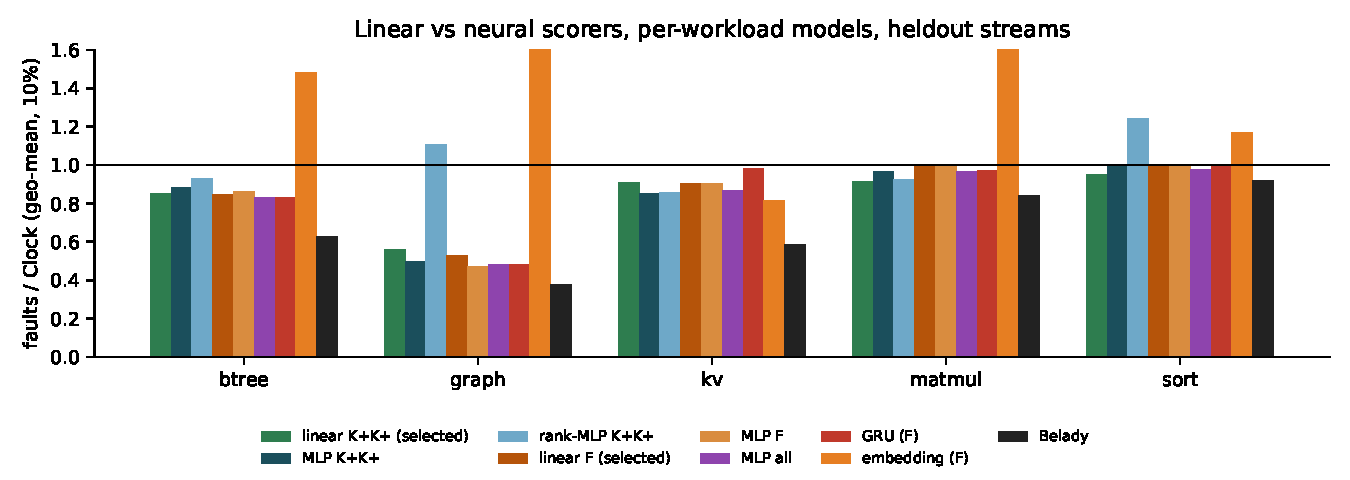
\includegraphics[width=.92\textwidth]{nn_heldout.pdf}

  \small
  A linear score is competitive with everything: MLP gains on kv and held-out graph only;
  the oracle GRU adds nothing; the cross-page embedding is catastrophic on
  btree/graph but best on held-out kv; the ranking loss did not help.
\end{frame}

\begin{frame}{Can it run without floating point?}
  \centering\tbl{quant_compact}

  \medskip
  \small With 8-bit weights and Q8 features every selected model is
  \good{within $\pm0.002$ of float} (most identical); 4-bit stays within $\sim$2\%.
  The policy runs in xv6 as trained --- no floating point.
\end{frame}

\begin{frame}{Does the training distribution matter? (one DAgger round)}
  \centering\tbl{dagger_compact}

  \medskip
  \small Re-recording under the model's own decisions and refitting does
  \warn{not} help: most selected models are unchanged or slightly worse. With
  stratified recording and probation, LRU-recorded decisions already cover
  the states these policies meet.
\end{frame}

% ------------------------------------------------------------------ close
\section{Conclusions}

\begin{frame}{Relation to Linux}
  \scriptsize
  \begin{tabular}{ll}
    \toprule
    Feature that won here & Linux already has \\
    \midrule
    \texttt{idle} (scans since last found accessed) & MGLRU generations; DAMON region age \\
    \texttt{sfreq} (scans found accessed) & DAMON \texttt{nr\_accesses}; MGLRU tiers \\
    \texttt{dirty} & \texttt{PG\_dirty} \\
    \texttt{refaults}, \texttt{rdist} & workingset shadow entries (\texttt{mm/workingset.c}) \\
    \texttt{rec}, \texttt{freq}, \texttt{sd} (oracle) & nothing without per-access instrumentation \\
    \bottomrule
  \end{tabular}

  \medskip\small
  The winning signals are ones Linux maintains; the score is a few integer
  multiply-adds per candidate in a scan the kernel already does.
\end{frame}

\begin{frame}{Takeaways}
  \small
  \begin{enumerate}
    \item On verified reference streams, a \textbf{linear score over 4--5
      kernel-observable features} beats xv6's best policy on all five workloads,
      on unseen seeds and unseen variants --- 2--32\% fewer faults (10--32\% on
      btree, graph, kv, matmul), up to 66\% fewer disk writes.
    \item \textbf{Oracle information buys almost nothing} over those features;
      \texttt{idle} (the kernel's own recency) carries most of the value.
    \item \textbf{Bigger models do not pay}: MLP, GRU, cross-page embedding, ranking loss
      are no better than linear except MLPs on kv and held-out graph.
    \item \textbf{Failure modes are real}: many feature sets are catastrophic, and the first
      training set taught models to evict the page being streamed. Validation-based
      selection and probation are part of the method, not details.
    \item The earlier graph and lzw results were measured on broken traces and are withdrawn.
  \end{enumerate}
\end{frame}

\begin{frame}{Next steps}
  \small
  \begin{enumerate}
    \item Implement the selected kernel+refault model as \texttt{VM\_POLICY\_ML} in
      \texttt{kernel/vmpage.c} with the integer path; pass the regression suite; measure
      faults, writes and eviction latency in xv6 itself.
    \item Choose weights per program or phase (the global model keeps less of the gain on matmul).
    \item Capacity-aware models for graph at 5\% and 20\%.
    \item Port the feature set to Linux MGLRU/DAMON signals.
  \end{enumerate}
\end{frame}

\end{document}
